% -----------------------------------------------------------------------------
\section{Purpose}
% -----------------------------------------------------------------------------

Many biological projects involve a communication in which one party requests that an experiment be executed by another party. 
Examples include remote collaborations, interdisciplinary projects, and cloud labs.
Experiment requests, however, involve a great deal of implicit knowledge about protocols, such as
the parameters that must be specified, the organisms that can be used, the instruments available, and constraints on when measurements can be taken.
As a result, 
requesting experiments typically requires a high degree of expert involvement and interpersonal communication, 
problems with requests are often detected late, 
and there are high costs associated with adding new protocols or onboarding new users.

\begin{figure}[htbp!]
\centering
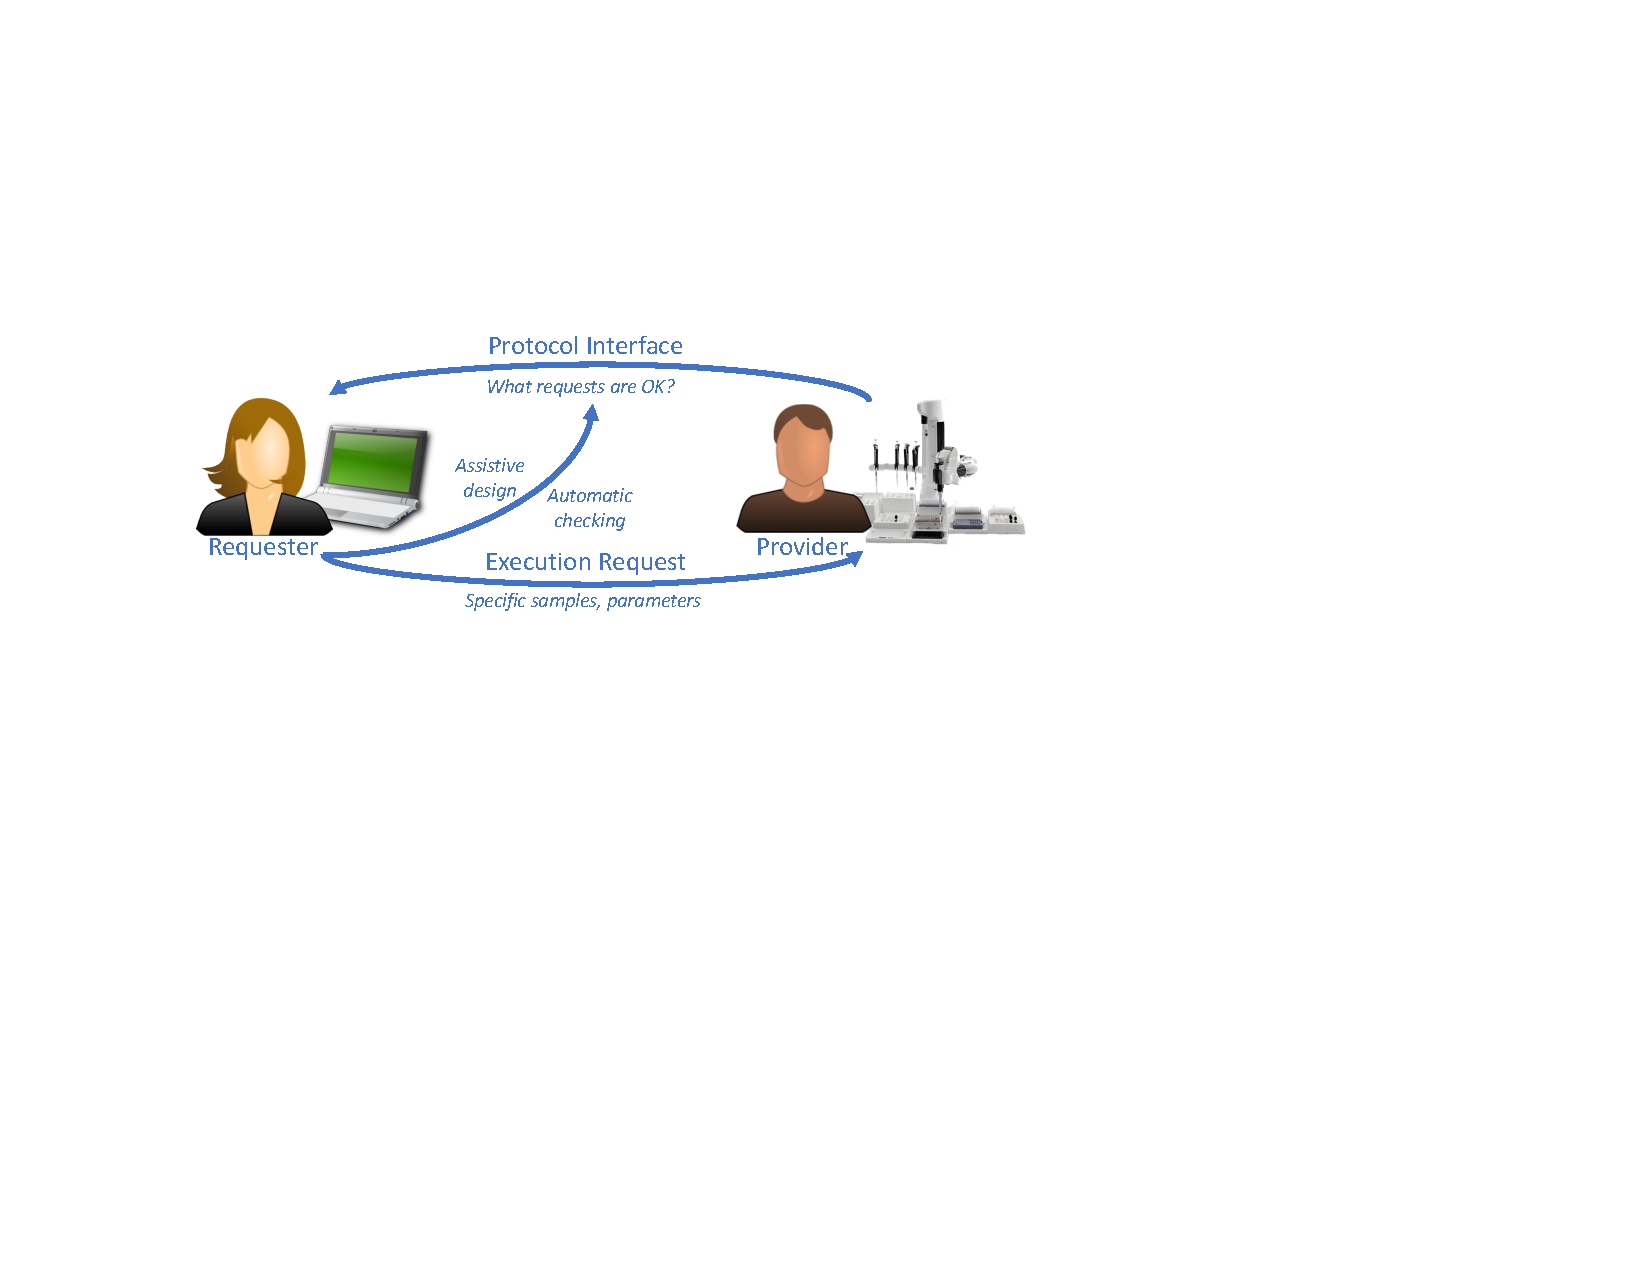
\includegraphics[width=0.8\textwidth]{figures/architecture.pdf}
\caption{OPIL connects experiment providers and requesters.}
\label{f:sequence}
\end{figure}

The Open Protocol Interface Language (OPIL) aims to address this problem by providing a data model to connect experiment providers and requesters.
Using OPIL, an experiment provider can provide a precise description of the protocols they offer, in terms of the options and constraints on the types of requests that can be made.
A requester can then use these interface descriptions to request the execution of a protocol on a specific set of samples with particular parameters.
OPIL can be applied both to automated protocols (e.g., via laboratory robotics or microfluidics) as well as to traditional human-executed ``paper'' protocols.

Where possible, OPIL builds on other existing standards.
In particular, OPIL uses the Synthetic Biology Open Language (SBOL) version 3~\cite{SBOL3} to describe biological samples in terms of combinations of strains, media, etc., and uses the Ontology of Units of Measure (OM) (\url{http://www.ontology-of-units-of-measure.org/resource/om-2}) to describe parameters with physical units.
Like these other standards, OPIL uses existing Semantic Web practices and resources, such as \emph{Uniform Resource Identifiers} (\opil{URI}s) and ontologies, to unambiguously identify and define biological system elements,
and to provide serialization formats for encoding this information in electronic data files.
This approach also allows OPIL to be extended with additional custom information for particular uses and deployments.

Note, however, that OPIL intentionally does not provide details about how the protocol works or guarantees about transfer or replicability of protocol executions. 
Likewise, OPIL is agnostic to any details of computer networking used to discover protocols or actually send requests.
OPIL focuses only on representing the minimal information for an unambiguous communication about requests to execute an offered protocol.

